\documentclass[conference,10pt]{IEEEtran}

\usepackage[T1]{fontenc}
\usepackage[utf8]{inputenc}
\usepackage{lmodern}
\usepackage{graphicx}
\usepackage{booktabs}
\usepackage{array}
\usepackage{amsmath}
\usepackage{amssymb}
\usepackage{float}
\usepackage{subcaption}
\usepackage{algorithm}
\usepackage{algpseudocode}
\usepackage{hyperref}
\usepackage{url}
\usepackage{tabularx}
\usepackage{multirow}
\usepackage{caption}

% Hyperlinks should be deactivated in the final PDF.
% The following command preserves URL formatting while avoiding active links.
\hypersetup{
    colorlinks=false,
    pdfborder={0 0 0}
}

\title{Classification of Network Traffic Using k-Nearest Neighbours and Decision Trees}

\author{
\IEEEauthorblockN{F. de Bruin}
\IEEEauthorblockA{
Student Number: 26990075 \\
Module Code: 741 \\
Email: \texttt{26990075@sun.ac.za}
}
}

\begin{document}
\pagestyle{plain}
\maketitle
\thispagestyle{plain}

\begin{abstract}
This report investigates multi-class network traffic classification with k-nearest neighbours and decision trees. The report uses a modified version of the UNSW-NB15 network traffic dataset. The dataset contains missing values, highly correlated features, unequal numeric ranges, and a skewed class distribution. The report examines the effect of these data quality issues on the two classifiers and discusses the preprocessing choices selected for each model. Stratified cross-validation and the macro-averaged F1-score support the evaluation under class imbalance. The final results show that the optimised decision tree provides the best balance between accuracy and macro-averaged F1-score. The results also show that preprocessing choices influence classifier behaviour strongly on this dataset.
\end{abstract}

\begin{IEEEkeywords}
network traffic classification, k-nearest neighbours, decision tree, preprocessing, class imbalance, cross-validation
\end{IEEEkeywords}

\section{Introduction}
Network traffic classification supports the identification of normal traffic and attack traffic in cyber security applications. Accurate classification supports network monitoring, intrusion detection, and threat analysis. This report examines two classical supervised learning methods, namely k-nearest neighbours and classification trees.

The report uses the edited UNSW-NB15 dataset provided as \texttt{networkTraffic.csv} on STEMlearn. The dataset contains numerical and nominal descriptive features, missing values, correlated features, outliers, and a heavily skewed class distribution. The target variable contains ten traffic categories. These characteristics make the dataset suitable for studying the relationship between preprocessing choices and classification performance.

The report applies a model-specific preprocessing strategy and uses only the transformations that are necessary for each learning method. The preprocessing for k-nearest neighbours differs from the preprocessing for classification trees. Distance-based learning reacts strongly to feature scale and redundant dimensions, whereas tree-based learning is less sensitive to feature magnitude. The empirical evaluation uses stratified cross-validation and reports accuracy together with the macro-averaged F1-score.

The remainder of the report is organised as follows. Section II presents the background of the dataset and the two classification methods. Section III describes the methodology and preprocessing decisions. Section IV presents the empirical procedure. Section V reports and discusses the experimental results. Section VI concludes the report. The appendices list acronyms and symbols used in the report.

\section{Background}
This section provides the conceptual basis for the report. The section introduces the classification task, the two learning methods, and the data quality issues that affect model behaviour. The section remains deliberately high level, because the methodological details are presented later.

\subsection{Network Traffic Classification}
Network traffic classification assigns each traffic instance to a class label. In this dataset, the class label represents one of ten traffic categories. The task is a multi-class classification problem with substantial class imbalance. Class imbalance means that majority classes contain far more observations than minority classes. Accuracy therefore does not provide a reliable view of classifier quality in this setting.

Network traffic classification supports intrusion detection and network monitoring in cyber security applications. Moustafa and Slay introduced the UNSW-NB15 dataset as a benchmark for modern intrusion detection research \cite{unsw}. The present report uses a modified version of that dataset.

The assignment dataset contains a number of remaining data quality issues from the original UNSW-NB15 features and from the edited STEMlearn version. The target classes remain skewed. The feature \texttt{id} is a unique identifier and has no predictive value. The features \texttt{proto}, \texttt{service}, and \texttt{state} are nominal rather than numeric. Missing values remain present in \texttt{service}. Many numeric features remain correlated. The numeric feature ranges differ substantially. Large outliers also remain present. These properties make the dataset a suitable test case for comparing learning methods that react differently to scale, redundancy, and imbalance.

\subsection{k-Nearest Neighbours}
k-nearest neighbours is an instance-based classification method \cite{knn}. The method assigns a class to an unseen observation by identifying the $k$ nearest training observations in feature space. The predicted class depends on the majority class among the nearest observations. Distance-weighted voting provides an alternative decision rule.

The method depends strongly on the distance metric and on the scale of the input features. Features with large numeric ranges can dominate the distance computation. Irrelevant and redundant features can also distort neighbourhood structure. Hastie, Tibshirani, and Friedman showed that feature scaling and feature selection are important for distance-based learning methods \cite{htf}. Missing values also complicate distance computation, because distance calculations require complete or imputed feature values. The present report therefore expects k-nearest neighbours to react strongly to the remaining missing values, the numeric scale differences, and the correlated features.

\subsection{Classification Trees}
A classification tree partitions the feature space by applying a sequence of if-then tests \cite{tree}. Each internal node represents a split on one feature. Each leaf node represents a predicted class. Classification trees are interpretable and can model non-linear decision boundaries.

Classification trees are less sensitive to feature scaling than distance-based methods. Breiman, Friedman, Olshen, and Stone showed that classification trees still react to noisy features, missing values, and class imbalance \cite{cart}. Unrestricted tree growth can also lead to overfitting. Tree depth and leaf-size constraints therefore act as important control parameters. The present report therefore expects classification trees to be less affected by feature scale than k-nearest neighbours, while still remaining sensitive to imbalance and noisy predictors.

\subsection{Data Quality Issues}
The dataset contains several data quality issues that remain relevant for the two learning methods. The feature \texttt{service} contains missing values. Several features are highly correlated, including feature pairs that convey overlapping information. The dataset contains outliers and feature ranges that differ widely. The class distribution is skewed. The features \texttt{proto}, \texttt{service}, and \texttt{state} are nominal. The \texttt{id} feature is a unique identifier and has no predictive value.

These issues affect the two learning methods differently. k-nearest neighbours reacts strongly to missing values, feature scale, redundant variables, and outliers. Classification trees are less sensitive to scale, but still require handling of missing values and noisy predictors. The report therefore applies model-specific preprocessing and avoids unnecessary transformations that do not improve the selected learning method.

\section{Methodology}
This section describes the practical approach that was followed to prepare the dataset and build the models. The section also explains the preprocessing choices for each learning method. Only transformations that were necessary for the selected learning method were applied.

\subsection{Dataset Preparation}
The dataset was loaded from the CSV file provided for the assignment. The value \texttt{?} was treated as a missing-value marker. The target variable was stored in the last column of the dataset. The identifier feature \texttt{id} was removed before modelling, because the identifier does not describe traffic behaviour and does not support prediction.

The nominal features \texttt{proto}, \texttt{service}, and \texttt{state} were treated as categorical variables. Missing values in \texttt{service} were retained as an explicit missing category during preprocessing. This choice preserved all observations and avoided the loss of a feature that still contained useful information.

\subsection{Preprocessing for k-Nearest Neighbours}
The k-nearest neighbours pipeline used median imputation for numeric features and most-frequent imputation for nominal features. The nominal features were encoded with one-hot encoding. Numeric features were scaled with robust scaling. Robust scaling was selected because the dataset contains outliers and highly skewed numeric distributions. Scaling was necessary for a distance-based method, because feature magnitude directly affects distance computation.

Highly correlated numeric features were removed in the optimised variant. This removal reduced redundancy in the distance calculation. The features \texttt{is\_ftp\_login} and \texttt{ct\_ftp\_cmd} contained invalid values greater than one. The optimised variant capped those values at one. That choice treated the features as binary indicators, which aligned with the feature descriptions provided for the dataset.

The k-nearest neighbours model used hyperparameter tuning for the number of neighbours, the voting rule, and the distance metric parameter. The goal was to identify a configuration that balanced bias and variance while remaining computationally feasible.

\subsection{Preprocessing for Classification Trees}
The classification tree pipeline used the same imputation and encoding steps as the k-nearest neighbours pipeline. Numeric scaling was not applied. Scaling was unnecessary for a classification tree because the tree splits on threshold values rather than on Euclidean distances.

The optimised classification tree variant also capped the invalid values in \texttt{is\_ftp\_login} and \texttt{ct\_ftp\_cmd}. Highly correlated features were not removed from the classification tree pipeline, because the tree tolerates redundancy better than k-nearest neighbours. The tree model used hyperparameter tuning for split criterion, maximum depth, minimum samples per split, minimum samples per leaf, and class weighting.

\subsection{Preprocessing Variants}
Two preprocessing variants were evaluated. The baseline variant used the minimum necessary preprocessing. The optimised variant used binary anomaly capping and removal of highly correlated numeric features for the k-nearest neighbours pipeline. The comparison between the two variants made it possible to observe the effect of extra cleaning on model performance.

\subsection{Model Construction}
Both classifiers were implemented in scikit-learn. The preprocessing steps were placed inside the modelling pipeline. This design prevents data leakage during cross-validation, because imputation, encoding, and scaling are learned only from the training folds within each split \cite{sklearn}.

\section{Empirical Procedure}
This section describes the evaluation strategy that was followed to compare the two models. The section also explains the performance measures and the control parameters used in the experiments.

\subsection{Cross-Validation Design}
Stratified cross-validation was used because the target distribution is skewed. Stratification preserves the class proportions in each fold. This design improves the reliability of the evaluation under class imbalance.

A fast validation run used a stratified sample of 50,000 observations and three folds. The purpose of the fast validation run was to verify that the full preprocessing and modelling pipeline functioned correctly before the final run. Three folds reduced runtime while still providing a class-balanced estimate of performance on a representative sample of the dataset.

The final run used the complete dataset and five folds. Five folds provided a stronger estimate of generalisation performance than three folds, while still keeping the computation manageable for the full dataset. The final run produced the main results used for reporting.

\subsection{Performance Measures}
Accuracy, macro-averaged F1-score, and weighted F1-score were used to evaluate the models. Accuracy gives the overall proportion of correct predictions. Macro-averaged F1-score averages the F1-score across classes with equal class weight. Weighted F1-score weights each class by its support.

Macro-averaged F1-score is the primary metric for this dataset, because the class distribution is highly imbalanced. Accuracy can appear high even when minority classes are classified poorly. Macro-averaged F1-score therefore provides a more balanced view of classifier performance.

\subsection{Control Parameters}
The k-nearest neighbours model was tuned over the number of neighbours, the voting rule, and the distance metric parameter. The classification tree model was tuned over the split criterion, maximum depth, minimum samples per split, minimum samples per leaf, and class weighting.

The optimised preprocessing variant was selected for the final comparison, because the validation run showed that the variant improved the balance of class-wise performance. The smaller grid in the fast validation run reduced runtime while still allowing comparison of the two learning methods. The final run used the complete dataset and the optimised preprocessing variant because that configuration produced the strongest macro-averaged F1-score.

\subsection{Experimental Workflow}
Algorithm~\ref{alg:workflow} summarises the empirical workflow.

\begin{algorithm}
\caption{Experimental workflow}
\label{alg:workflow}
\begin{algorithmic}[1]
\State Load the dataset from the CSV file
\State Remove the identifier feature
\State Encode nominal features
\State Impute missing values
\State Apply model-specific preprocessing
\State Tune the control parameters by stratified cross-validation
\State Evaluate accuracy, macro-averaged F1-score, and weighted F1-score
\State Compare k-nearest neighbours and classification trees
\end{algorithmic}
\end{algorithm}

\section{Results and Discussion}
This section reports the results of the final run and discusses the implications of the findings. The section uses the optimised preprocessing variant as the final comparison basis.

\subsection{Overall Model Comparison}
Table~\ref{tab:model_comparison} presents the final summary values for the optimised variant. The decision tree achieves the highest macro-F1-score. The k-nearest neighbours model achieves the highest accuracy, but the macro-F1-score is lower. The lower macro-F1-score indicates weaker balanced performance across the ten classes.

\begin{table}[H]
\caption{Overall model comparison}
\label{tab:model_comparison}
\centering
\begin{tabular}{lccc}
\toprule
Model & Accuracy & Macro-F1 & Weighted-F1 \\
\midrule
k-Nearest Neighbours & 0.7859 & 0.5075 & 0.7832 \\
Decision Tree & 0.7675 & 0.5876 & 0.7951 \\
\bottomrule
\end{tabular}
\end{table}

The decision tree is the preferred model for this dataset, because the evaluation metric that reflects class balance is higher. The result is consistent with the skewed class distribution. The k-nearest neighbours model favours the majority classes more strongly, which inflates accuracy but does not improve balanced class performance.

\subsection{Class-wise Performance}
Table~\ref{tab:dt_classwise} shows the class-wise classification report for the optimised decision tree. The model performs well on the largest classes, especially classes 0, 1, 4, 6, and 9. The model also achieves strong performance on class 7, which contains only 174 observations. The minority classes 2 and 5 remain difficult to classify. The same pattern appears in the k-nearest neighbours results, although the class-wise balance is weaker.

\begin{table}[H]
\caption{Decision tree class-wise performance}
\label{tab:dt_classwise}
\centering
\begin{tabular}{lccc}
\toprule
Class & Precision & Recall & F1-score \\
\midrule
0 & 0.9627 & 0.8221 & 0.8868 \\
1 & 0.8510 & 0.7864 & 0.8174 \\
2 & 0.0501 & 0.2709 & 0.0846 \\
3 & 0.3535 & 0.5543 & 0.4317 \\
4 & 0.8630 & 0.5134 & 0.6438 \\
5 & 0.0734 & 0.2122 & 0.1090 \\
6 & 0.5647 & 0.7464 & 0.6430 \\
7 & 0.5360 & 0.8563 & 0.6593 \\
8 & 0.4895 & 0.8213 & 0.6134 \\
9 & 0.9945 & 0.9799 & 0.9872 \\
\bottomrule
\end{tabular}
\end{table}

The minority classes are difficult to classify because the available evidence is limited. Class 2 and class 5 receive low F1-scores. The model therefore has difficulty learning stable decision regions for those classes. The result is expected under severe imbalance.

\subsection{Effect of Preprocessing}
The optimised variant improves the modelling pipeline in two ways. First, the capping of invalid binary values removes values that do not match the feature definition. Second, the removal of highly correlated numeric features reduces redundancy in the k-nearest neighbours distance calculation. These changes improve the interpretability of the preprocessing strategy and support the stronger macro-F1-score of the decision tree.

The decision tree benefits from the absence of unnecessary scaling. The model also benefits from class weighting during tuning. The class weights help the tree pay more attention to minority classes. The effect is visible in the non-zero recall values for the smaller classes.

\subsection{Graph-Based Discussion}
Figure~\ref{fig:model_comparison} compares the two models across the main evaluation metrics. Figure~\ref{fig:dt_f1} and Figure~\ref{fig:knn_f1} show the class-wise F1-scores. Figure~\ref{fig:dt_cm} and Figure~\ref{fig:knn_cm} show the normalised confusion matrices.

\begin{figure}[H]
    \centering
    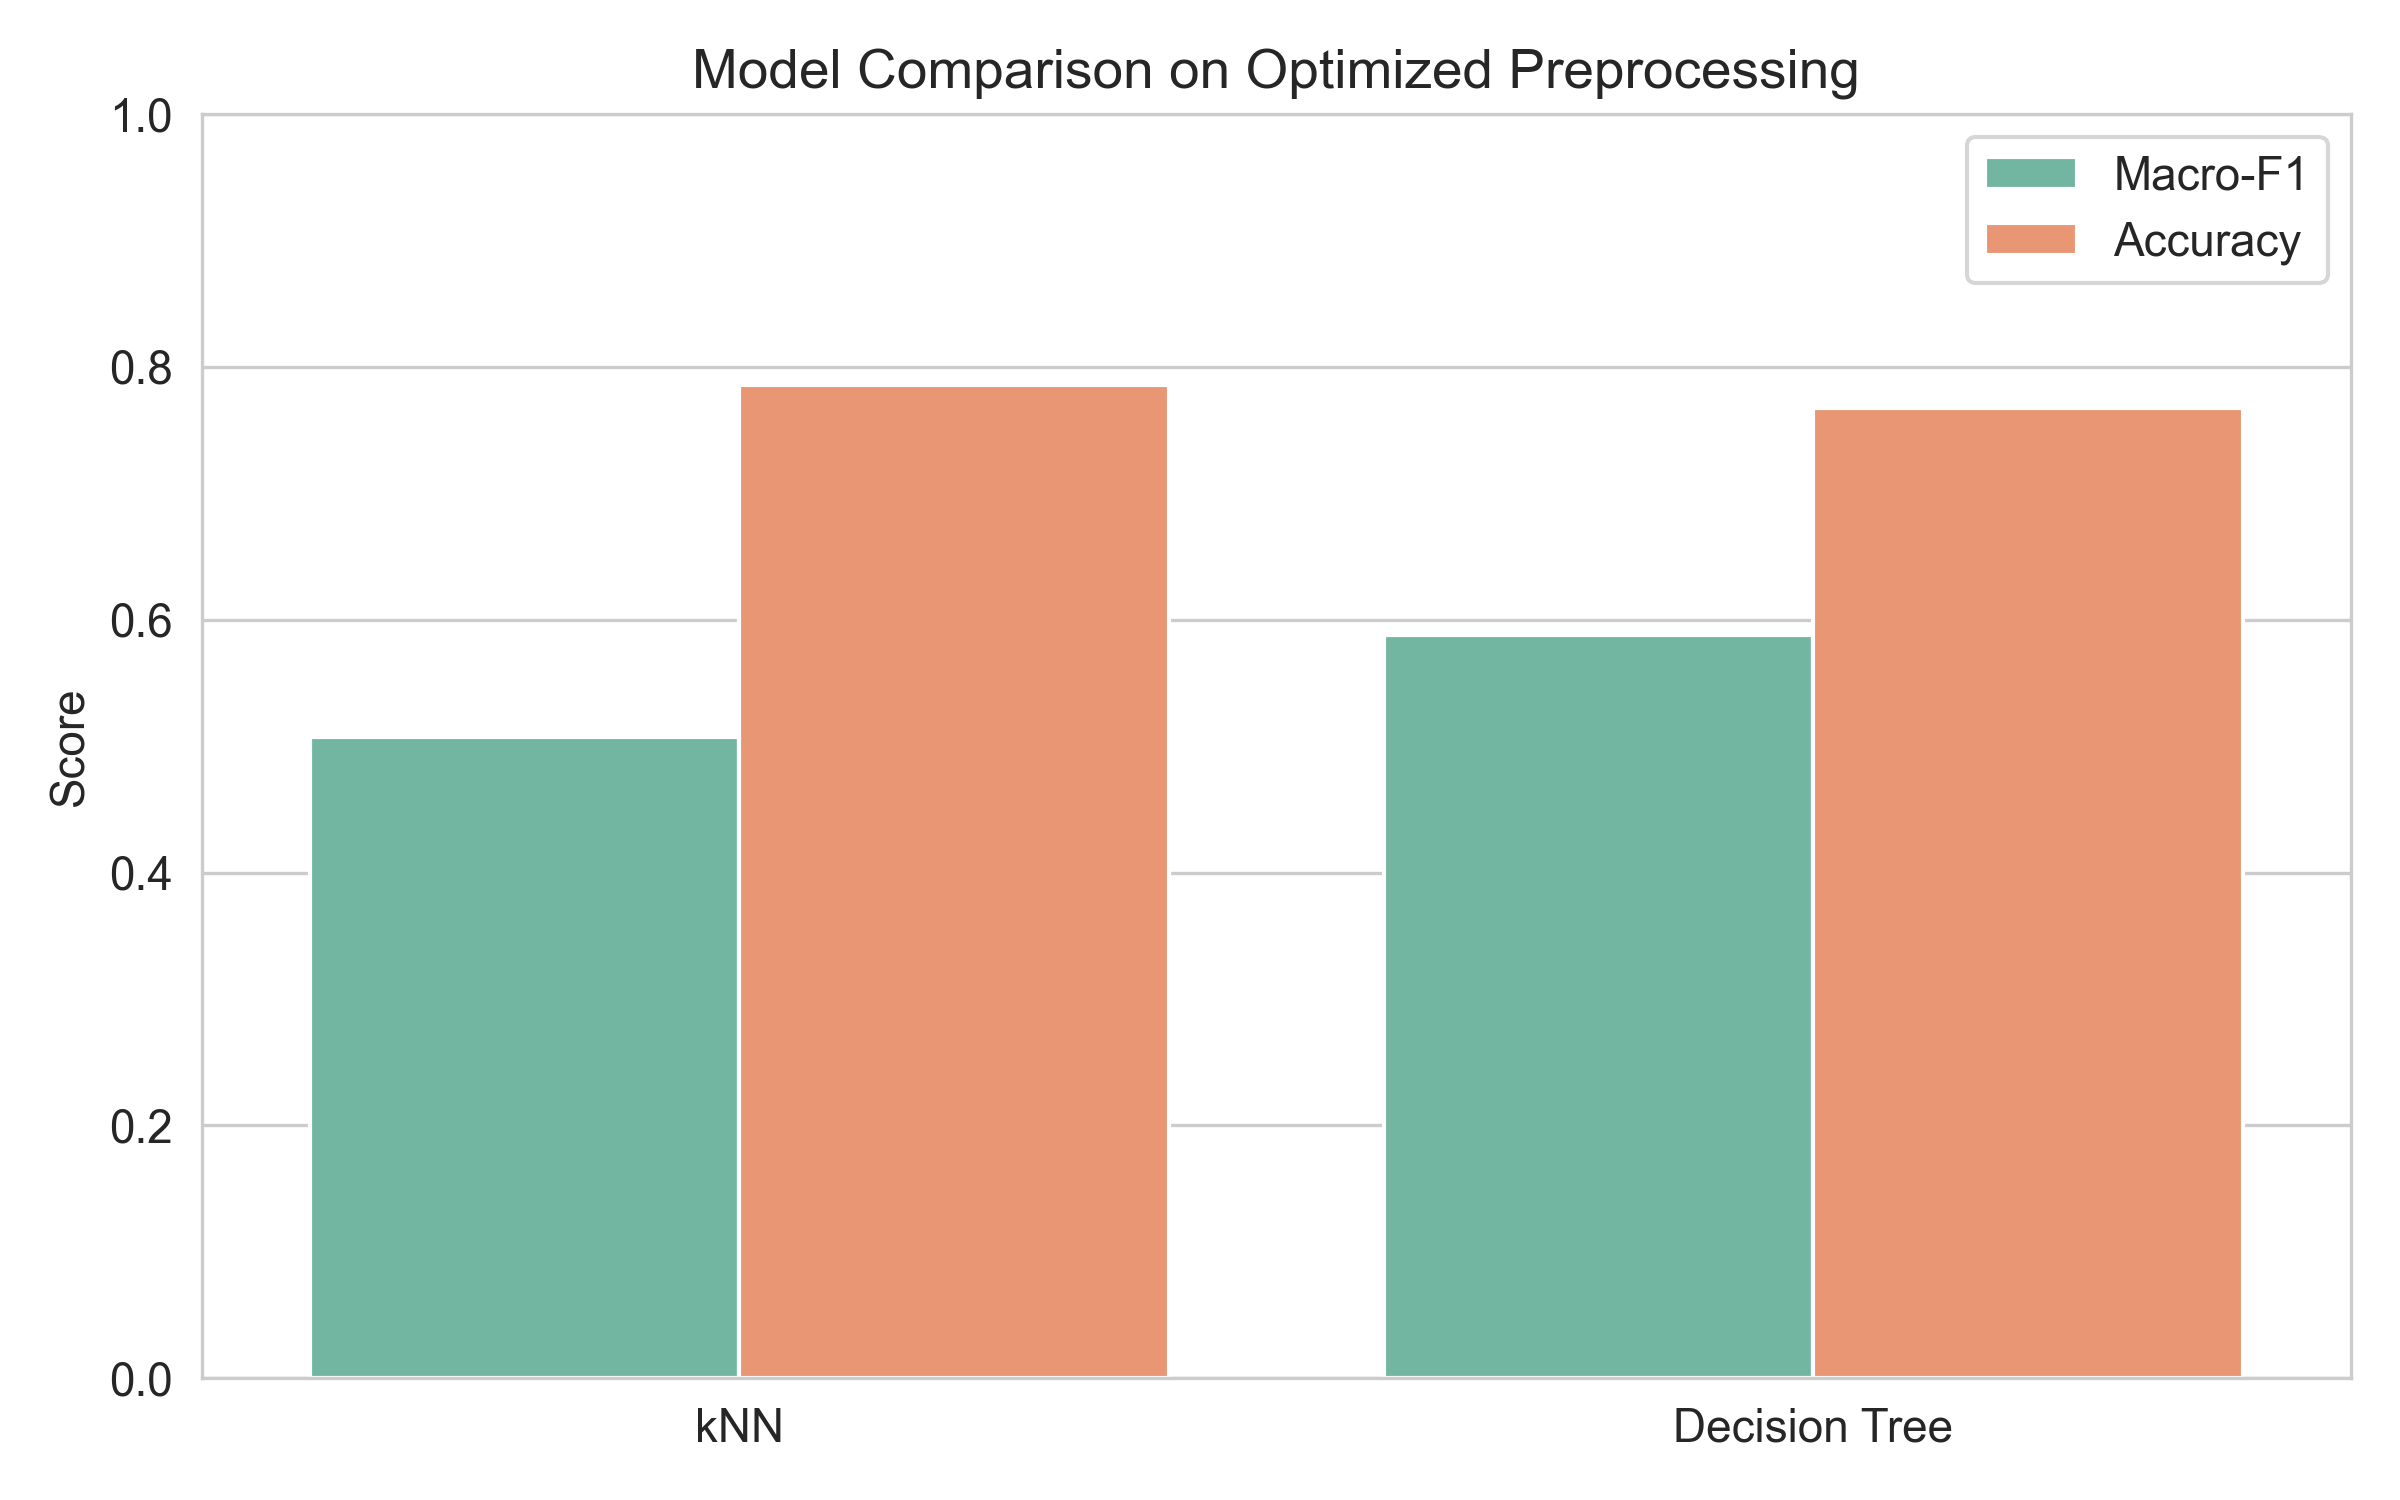
\includegraphics[width=\linewidth]{model_results/graphs/model_comparison.png}
    \caption{Model comparison}
    \label{fig:model_comparison}
\end{figure}

\begin{figure}[H]
    \centering
    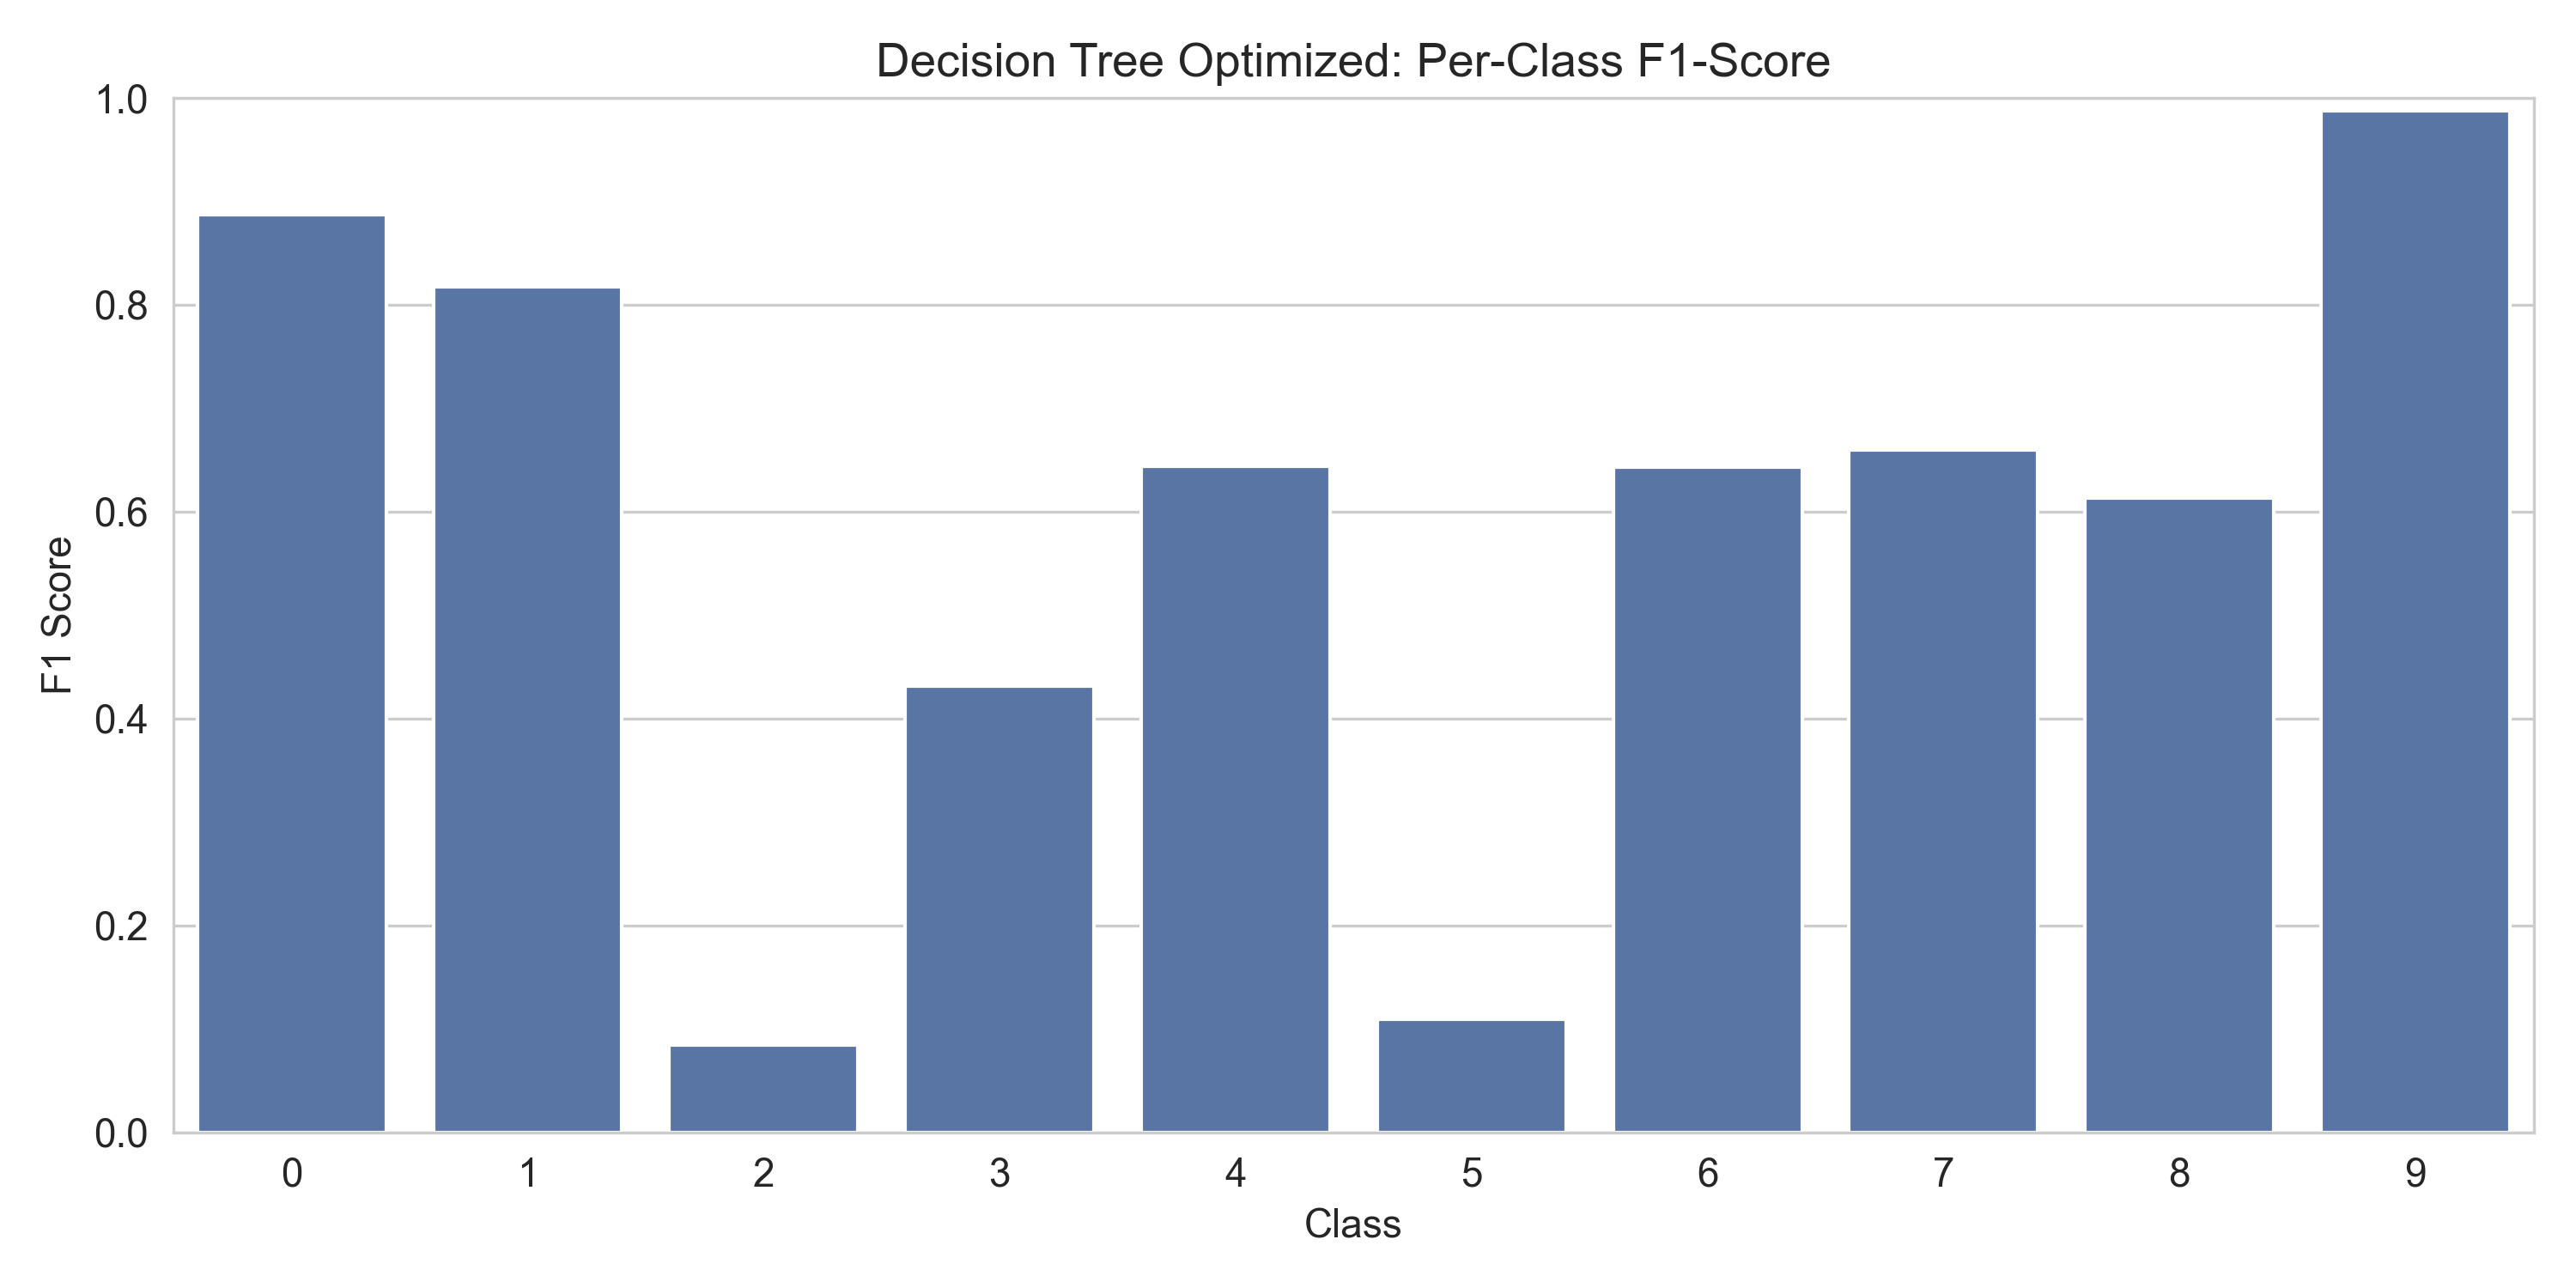
\includegraphics[width=\linewidth]{model_results/graphs/decision_tree_optimized_f1.png}
    \caption{Decision tree class-wise F1-scores}
    \label{fig:dt_f1}
\end{figure}

\begin{figure}[H]
    \centering
    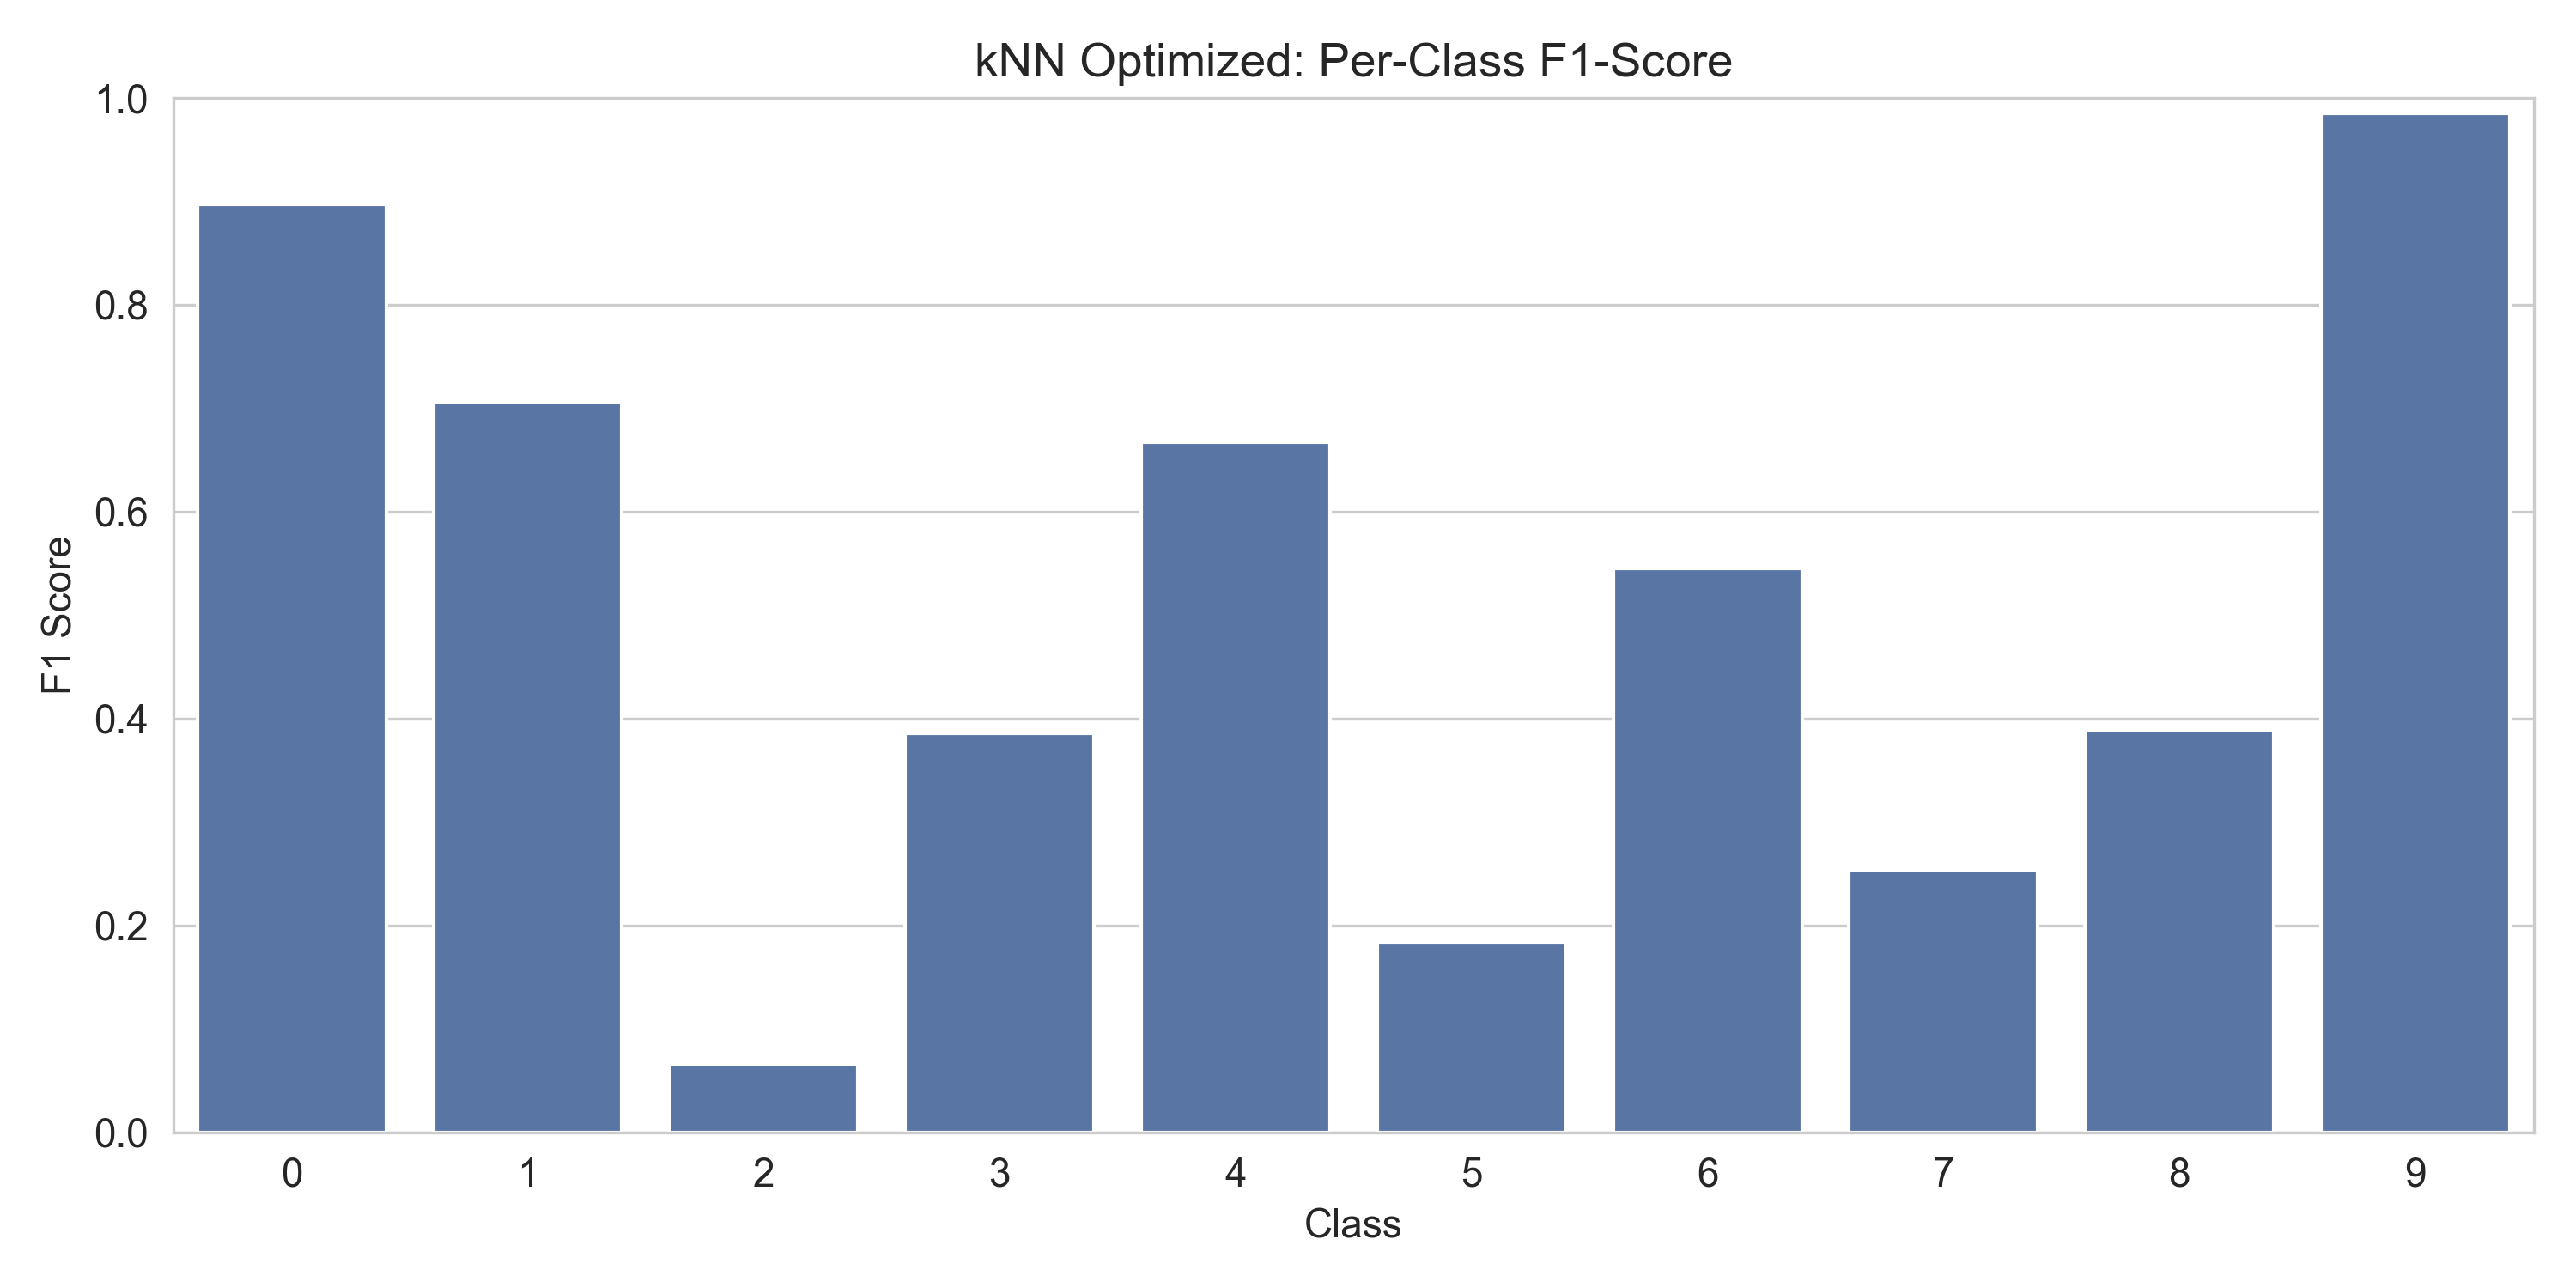
\includegraphics[width=\linewidth]{model_results/graphs/knn_optimized_f1.png}
    \caption{k-nearest neighbours class-wise F1-scores}
    \label{fig:knn_f1}
\end{figure}

\begin{figure}[H]
    \centering
    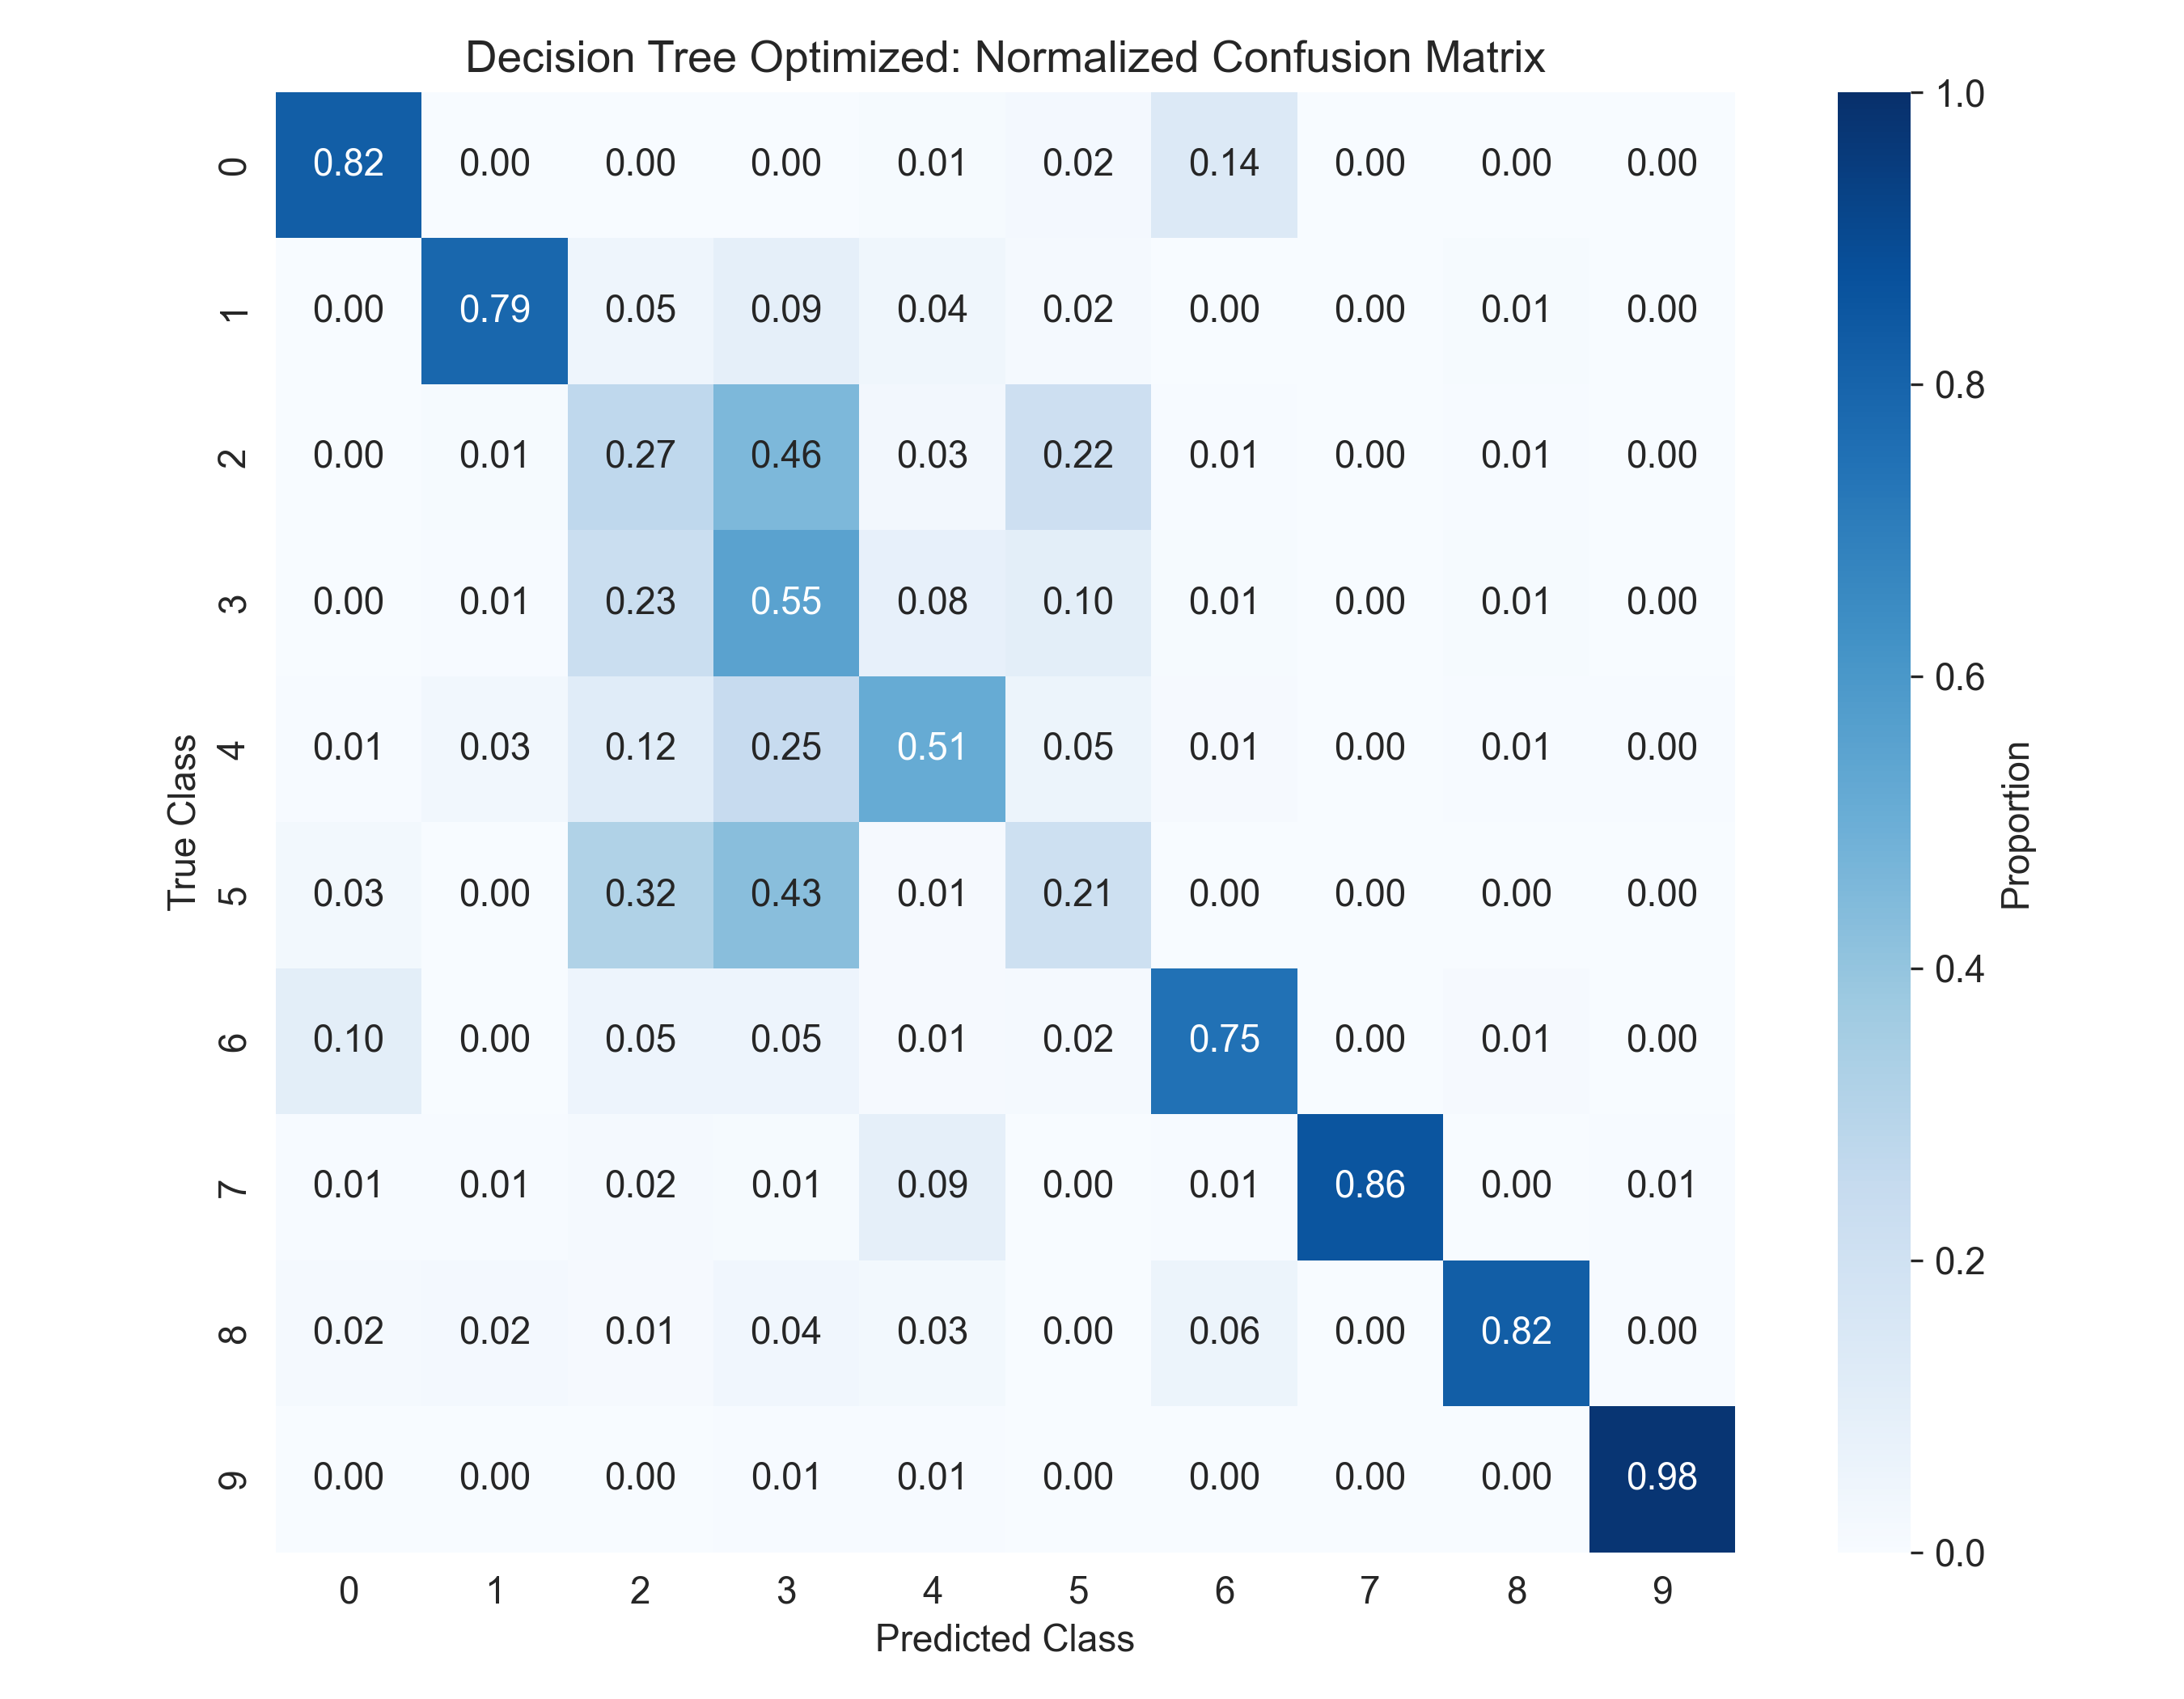
\includegraphics[width=\linewidth]{model_results/graphs/decision_tree_optimized_cm_norm.png}
    \caption{Decision tree normalised confusion matrix}
    \label{fig:dt_cm}
\end{figure}

\begin{figure}[H]
    \centering
    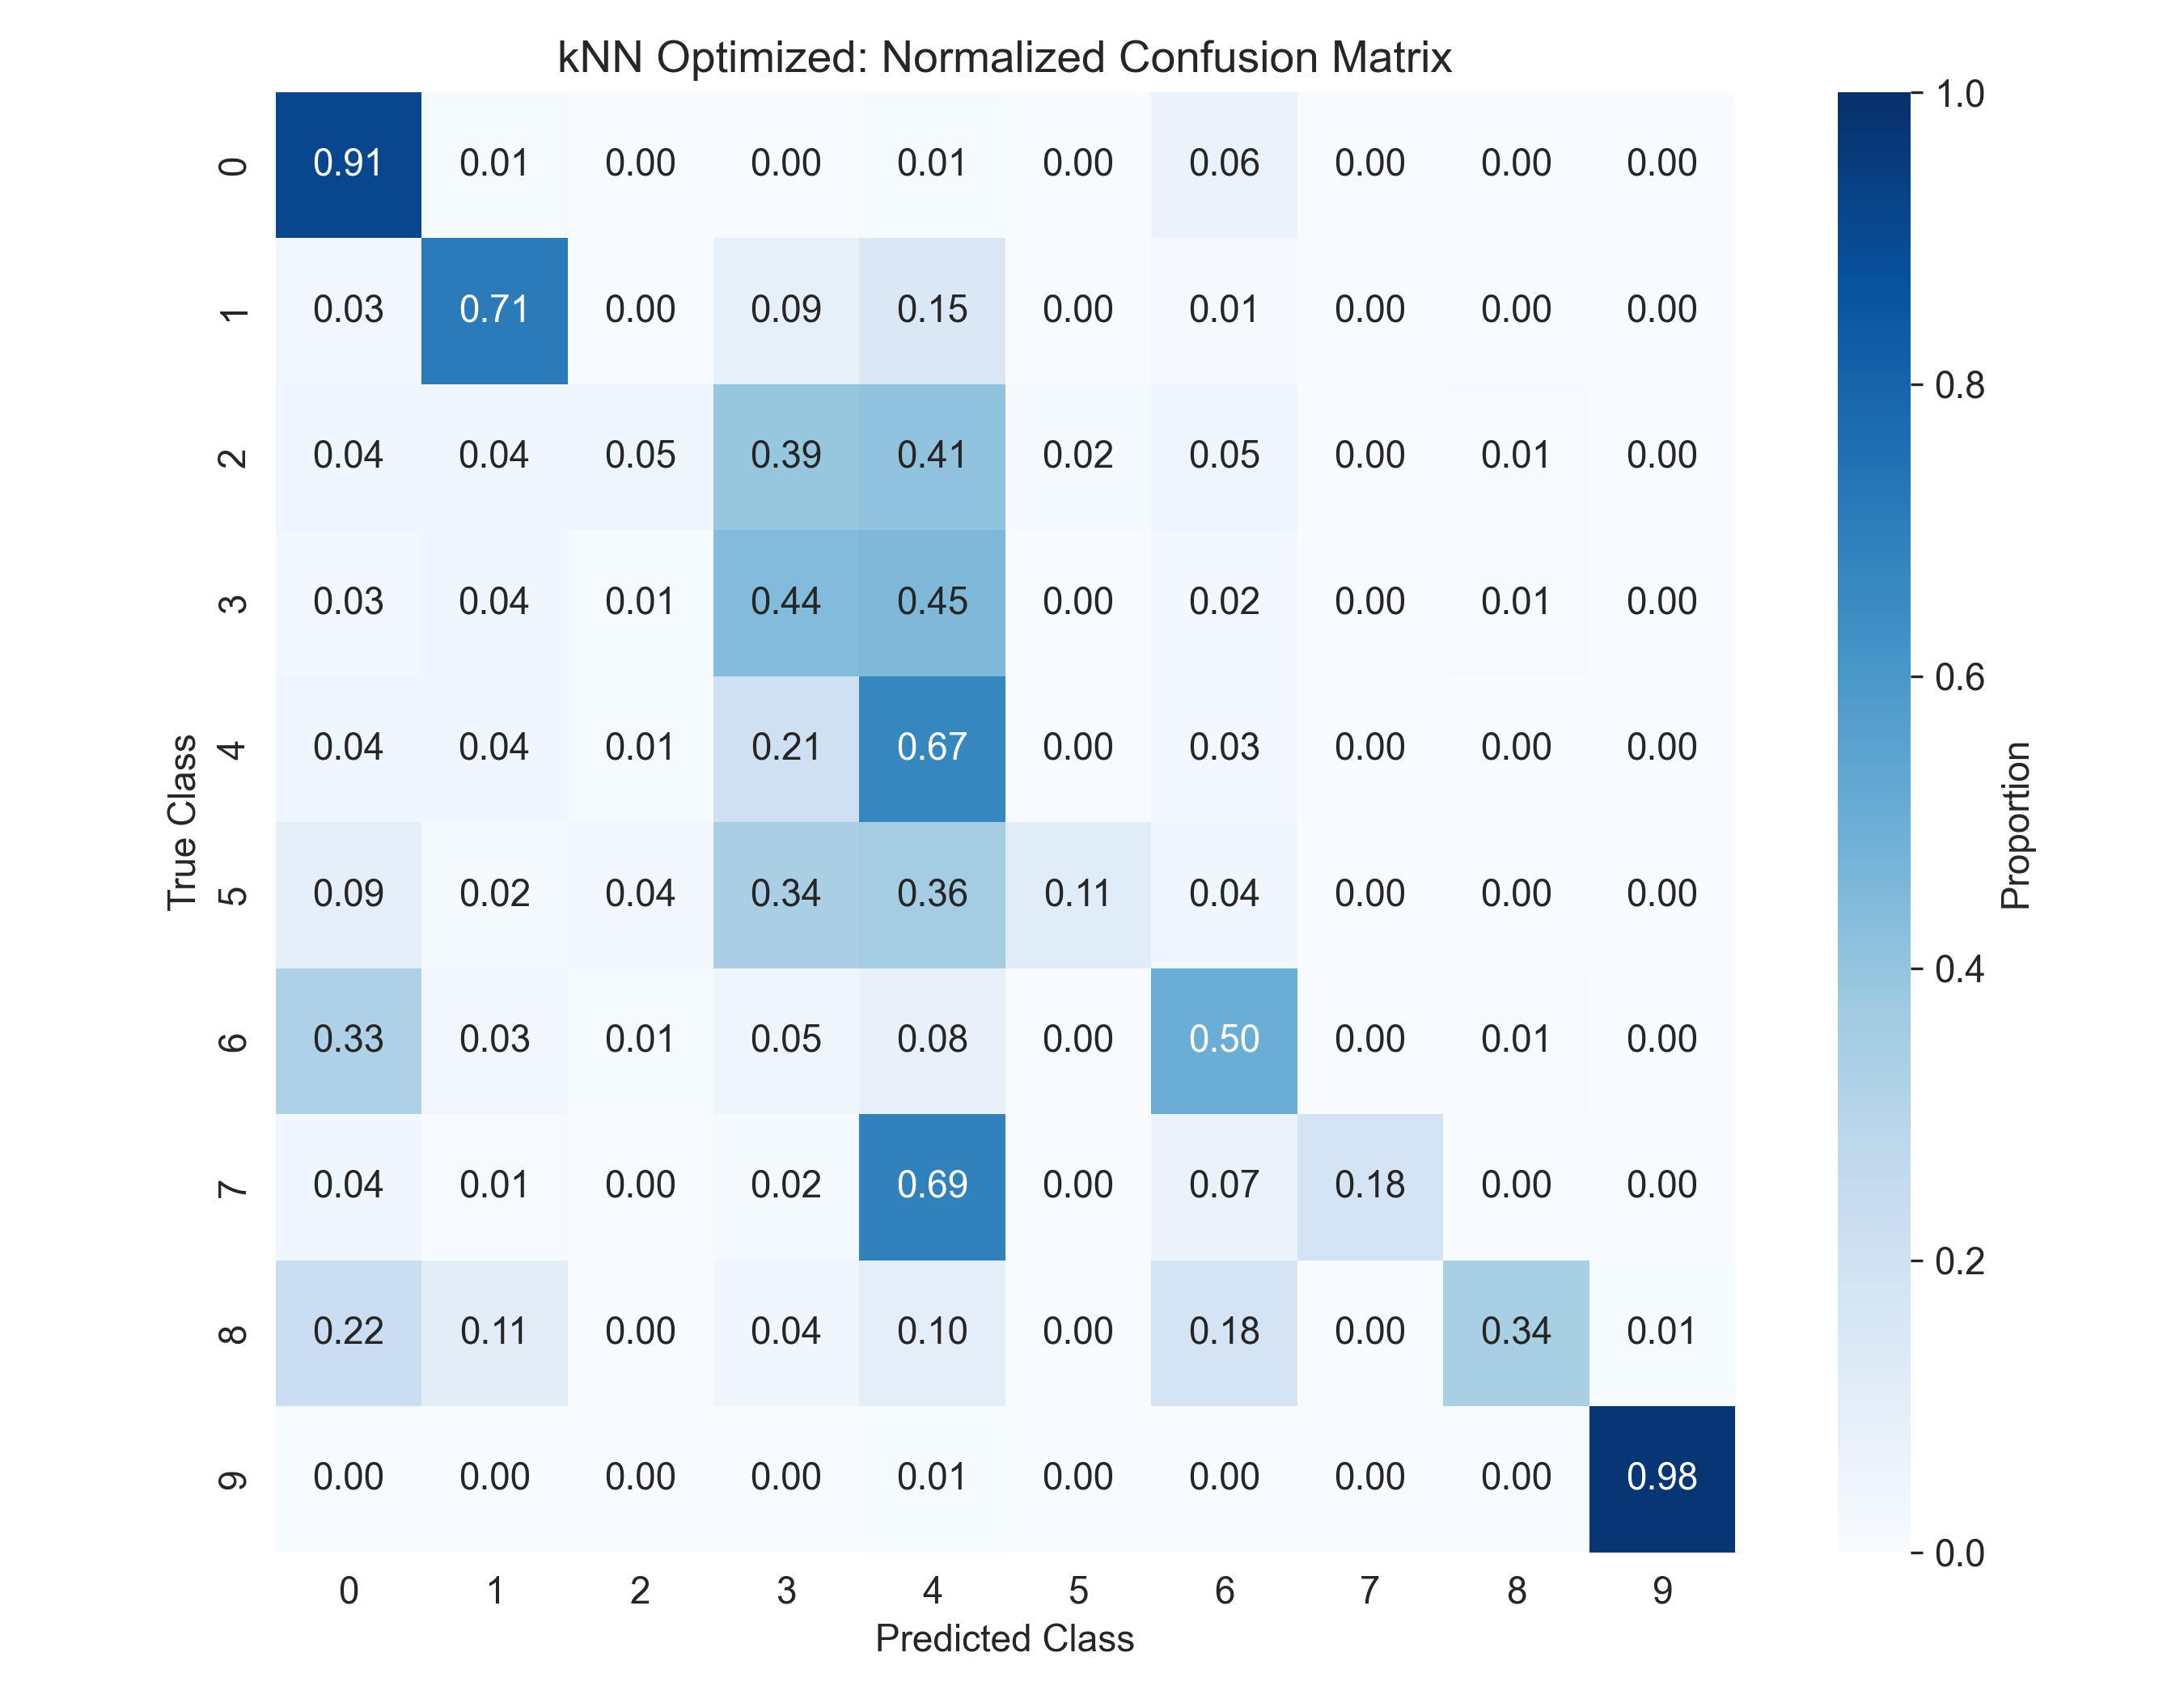
\includegraphics[width=\linewidth]{model_results/graphs/knn_optimized_cm_norm.png}
    \caption{k-nearest neighbours normalised confusion matrix}
    \label{fig:knn_cm}
\end{figure}

The model comparison figure shows that the decision tree has the stronger macro-F1-score, while k-nearest neighbours has the slightly higher accuracy. The class-wise figures show that both models perform well on the dominant classes. The decision tree performs better than k-nearest neighbours on the smaller classes 3, 5, 7, and 8. The k-nearest neighbours model shows a stronger tendency to misclassify minority classes as classes 3, 4, and 6.

The normalised confusion matrices provide a clearer view of class-wise behaviour than the raw counts. The decision tree matrix shows strong diagonal structure for classes 0 and 9. The k-nearest neighbours matrix also shows strong diagonal structure for class 9, but the matrix contains more confusion between classes 2, 3, 4, 5, 6, 7, and 8. The matrices confirm that minority classes remain difficult to separate from neighbouring attack categories.

The k-nearest neighbours matrix shows especially strong confusion for class 8, which is frequently predicted as classes 0, 1, 4, 6, or 8. The decision tree matrix shows that class 8 is also difficult, but the tree still achieves a better overall class-wise balance. The decision tree also separates class 7 more effectively than k-nearest neighbours.

The figures support the numerical results. The model comparison figure confirms that the decision tree is the better model under macro-averaged evaluation. The per-class figures confirm that the decision tree provides a more balanced distribution of F1-scores across the classes. The confusion matrices show that the class imbalance remains a major limitation, even after preprocessing.

\subsection{Summary of Findings}
The final comparison shows that the decision tree is the preferred model for this dataset. The model is more balanced across classes and achieves the highest macro-F1-score. The k-nearest neighbours model achieves slightly higher accuracy, but the class-balanced performance is weaker. The report therefore selects the decision tree as the most suitable classifier for the assignment.

\section{Conclusion}
This report investigated network traffic classification using k-nearest neighbours and decision trees. The study used the modified UNSW-NB15 dataset and applied model-specific preprocessing. The dataset contained missing values, redundancy, unequal feature scales, and severe class imbalance.

The empirical results showed that the optimised decision tree performed best overall. The decision tree achieved the highest macro-F1-score and the strongest balance across classes. The k-nearest neighbours model achieved slightly higher accuracy, but the lower macro-F1-score indicated weaker performance on the imbalanced class structure.

The study showed that preprocessing choices had a strong effect. The removal of redundant features and the capping of invalid binary values supported the final preprocessing strategy. The decision tree was more suitable for the dataset than k-nearest neighbours under the chosen evaluation criteria. The final results supported the use of macro-F1-score as the primary metric for skewed multi-class classification problems.

\newpage

\appendices
\section{Acronyms}
\begin{tabular}{ll}
CV & Cross-validation \\
F1 & Harmonic mean of precision and recall \\
kNN & k-nearest neighbours \\
ML & Machine learning \\
UNSW-NB15 & University of New South Wales Network Benchmark 15 \\
\end{tabular}

\bigskip

\section{Symbols}
\begin{tabular}{ll}
$k$ & Number of nearest neighbours \\
$X$ & Feature matrix \\
$y$ & Target vector \\
\end{tabular}

\bigskip

\begin{thebibliography}{99}

\bibitem{cart}
L. Breiman, J. H. Friedman, R. A. Olshen, and C. J. Stone, \textit{Classification and Regression Trees}. Belmont, CA, USA: Wadsworth, 1984.

\bibitem{htf}
T. Hastie, R. Tibshirani, and J. Friedman, \textit{The Elements of Statistical Learning: Data Mining, Inference, and Prediction}. New York, NY, USA: Springer, 2009.

\bibitem{knn}
T. M. Cover and P. E. Hart, ``Nearest neighbor pattern classification,'' \textit{IEEE Transactions on Information Theory}, vol. 13, no. 1, pp. 21--27, 1967.

\bibitem{sklearn}
F. Pedregosa et al., ``Scikit-learn: Machine learning in Python,'' \textit{Journal of Machine Learning Research}, vol. 12, pp. 2825--2830, 2011.

\bibitem{tree}
J. R. Quinlan, \textit{C4.5: Programs for Machine Learning}. San Francisco, CA, USA: Morgan Kaufmann, 1993.

\bibitem{unsw}
N. Moustafa and J. Slay, ``UNSW-NB15: A comprehensive data set for network intrusion detection systems,'' in \textit{Proceedings of the Military Communications and Information Systems Conference}, 2015.

\end{thebibliography}

\end{document}